\clearpage
\section*{Section C (Circuit Interruption): Question 1}
\addcontentsline{toc}{section}{Section C (Circuit Interruption): Question 1}

The case below (figure on the left) represents a typical short-circuit fault in transmission lines and the breaker operation for line interruption. The equivalent circuit is shown in the figure on the right.

\begin{figure}[h!]
    \centering
    \begin{minipage}{0.45\textwidth}
        \centering
        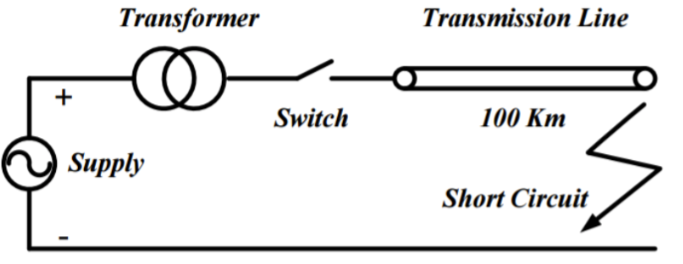
\includegraphics[width=\textwidth]{figures/figure-C-circuit-left.png}
        \caption{Transmission line with short-circuit fault}
        \label{fig:c01_circuit_left}
    \end{minipage}
    \hfill
    \begin{minipage}{0.45\textwidth}
        \centering
        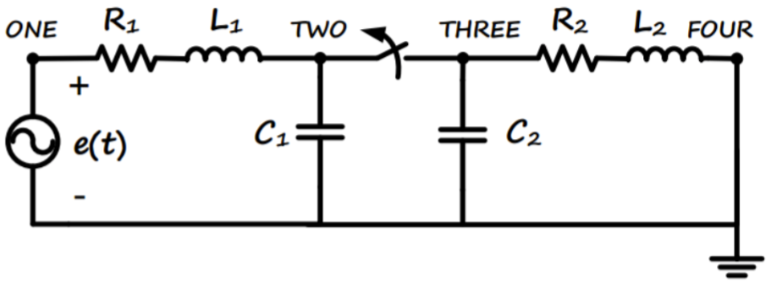
\includegraphics[width=\textwidth]{figures/figure-C-circuit-right.png}
        \caption{Equivalent circuit representation}
        \label{fig:c01_circuit_right}
    \end{minipage}
\end{figure}

On the left-hand side of the switch/breaker, we have the source voltage and a resistance and inductance representing the supply system combined with the transformer. The capacitor to the left of the breaker represents the combined substation capacitance due to the substation busbars. On the right-hand side of the breaker, we have the transmission line parameters: resistance, inductance, and capacitance represented as simple lumped parameters, where the right side is short-circuited due to the fault, assuming that the fault has already been applied. We have assumed a single-phase circuit here for simplicity. The parameters of the circuit below are: $e(t) = 230\times\cos(\omega t)$ kV, $\omega=377$ rad/s, $R_1=3\Omega$, $L_1=350$ mH, $R_2=50\Omega$, $L_2=100$ mH, $C_1=10$ nF, $C_2=600$ nF. Assume that the system is operating with zero initial conditions and the breaker is initially closed. At $t=8$ ms, the breaker is commanded to open the line, but it will not actually open until the current passes through zero. The study period is from $t=0$ to $t=20$ ms.

1) Choose an appropriate simulation time-step size $\Delta t$ (assuming the Trapezoidal integration rule) according to the time constants in the circuit. For this, evaluate the approximate resonant frequencies analytically before and after the breaker operation.

\noindent\rule{\textwidth}{0.4pt}

% Your solution here